\PassOptionsToPackage{unicode}{hyperref}
\documentclass[aspectratio=1610, 9pt]{beamer}

% Load packages you need here
\usepackage{polyglossia}
\setmainlanguage{english}

\usepackage{csquotes}
    

\usepackage{amsmath}
\usepackage{amssymb}
\usepackage{mathtools}

\usepackage{hyperref}
\usepackage{bookmark}

% load the theme after all packages

\usetheme[
  showtotalframes, % show total number of frames in the footline
]{tudo}

% Put settings here, like
\unimathsetup{
  math-style=ISO,
  bold-style=ISO,
  nabla=upright,
  partial=upright,
  mathrm=sym,
}

\title{Generation and time-resolved detection of
terahertz radiation}
\author[M.~Koch]{Max Koch}
\institute[AG Wang]{Arbeitsgruppe Wang \\  Fakultät Physik}
\titlegraphic{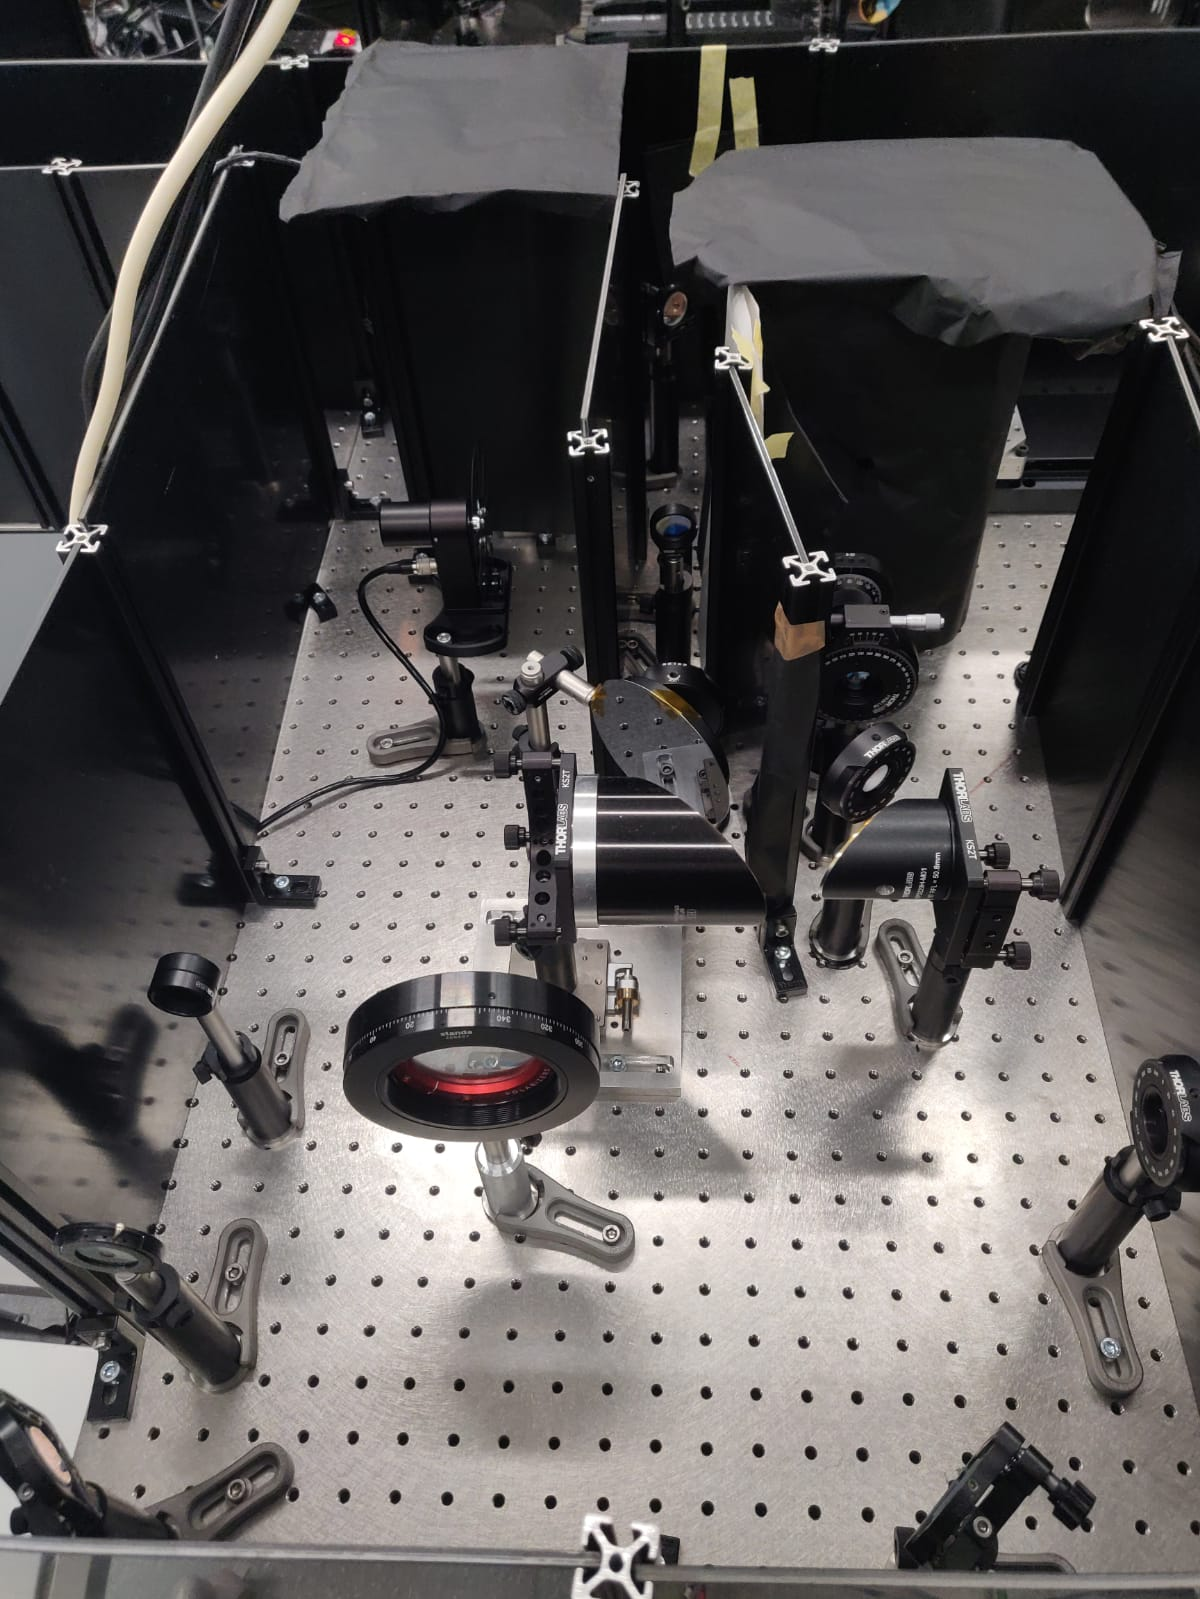
\includegraphics[width=0.2\textwidth]{images/setup.jpeg}}


\begin{document}

\maketitle

\section{Intro}

\begin{frame}{The Gap}
  \subsection{The spectrum}
%    \icludegraphic{content/spectrum.png}
\end{frame}

\begin{frame}{Outline}
  \tableofcontents
\end{frame}

\begin{frame}{Terahertz}
  So why do we need terahertz radiation?
  \begin{itemize}
    \item medizin
    \item security
    \item data transmission \& saving
    \item physics
  \end{itemize}
\end{frame}

\section{Setup}

\begin{frame}{Okay THz good, but how?}
  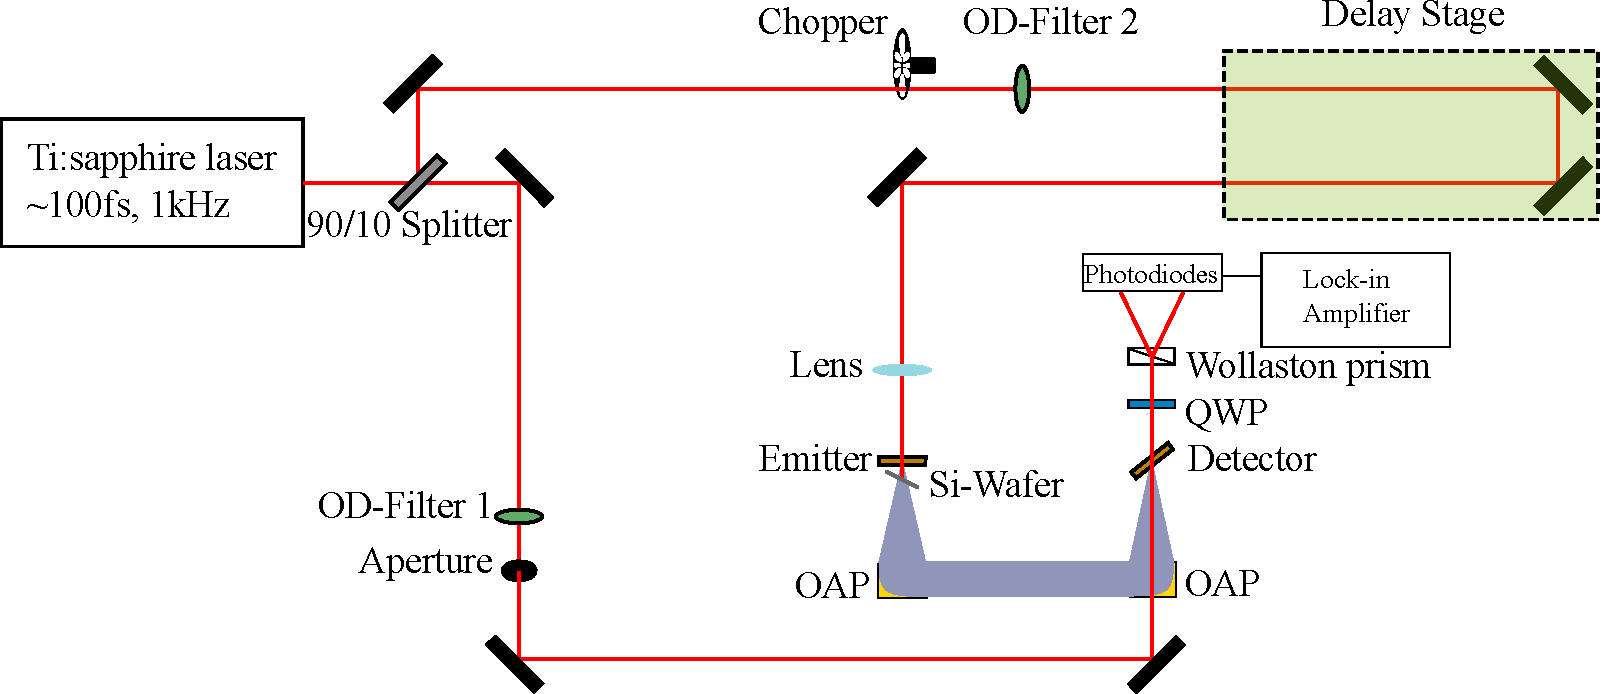
\includegraphics[width=\textwidth]{images/Aufbau.pdf}
\end{frame}

\section{Theory}
\begin{frame}{Optical-rectification}
  So what's the theory behind terahertz generation?
  \begin{itemize}
    \item Two photons go in
    \item Higher energy level
    \item two photon emission 
    \item energy drops to gorundstate
  \end{itemize}
  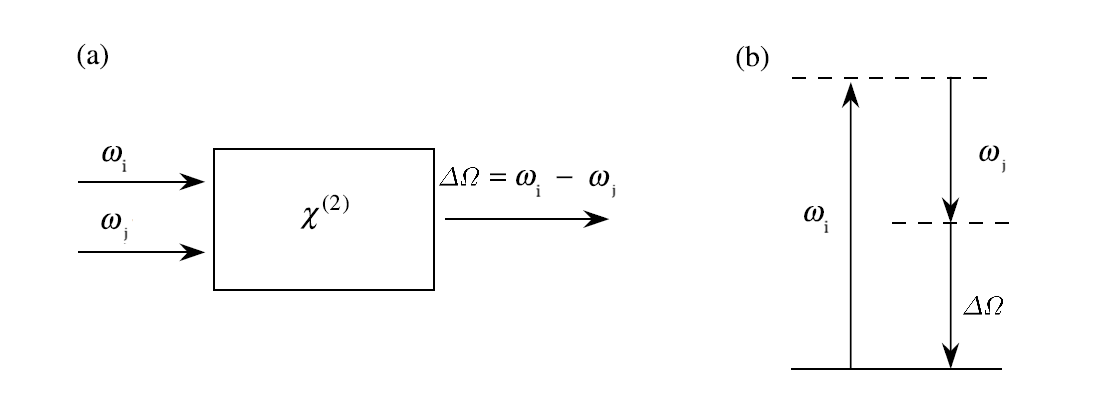
\includegraphics[width=0.5\textwidth]{images/diffrence_frequency_mixing.PNG}
\end{frame}

\begin{frame}{Electro-optic sampling}
  And how to detect it?

\end{frame}

\begin{frame}{Coherence-length}

\end{frame}

\section{Results}

\end{document}
